\chapter{Principal Component Analysis}
\label{ch:pca}

Which of the following three scatter plots (showing x vs. y, x vs. z and y vs. z) for the same three-dimensional data gives us the best picture about the actual layout of the data in space?

\begin{figure*}[h]
    \centering
    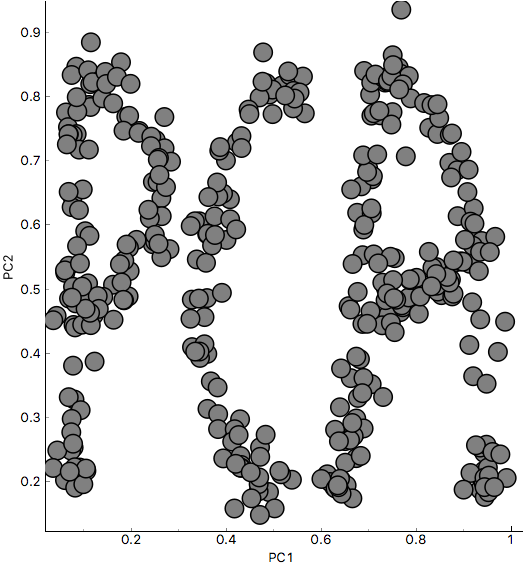
\includegraphics[scale=0.25]{pca1.png}
    \hspace{0.5cm}
    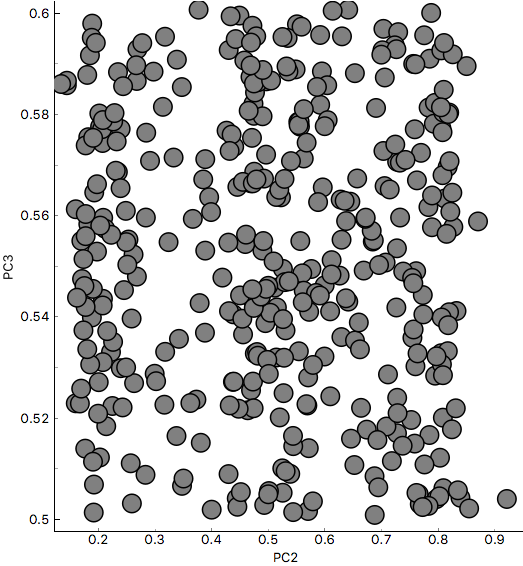
\includegraphics[scale=0.25]{pca2.png}
    \hspace{0.5cm}
    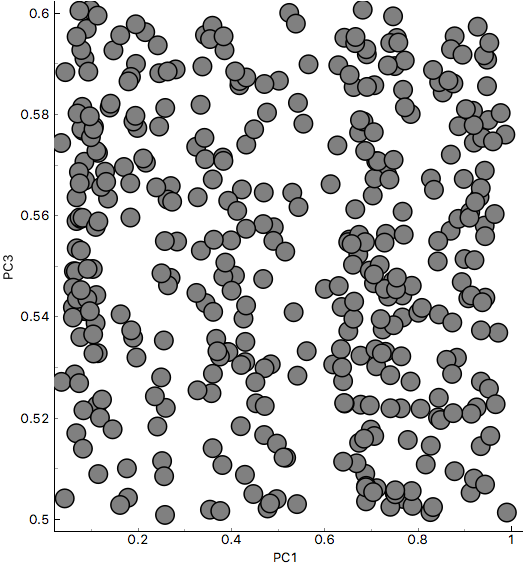
\includegraphics[scale=0.25]{pca3.png}
    \caption{$\;$}
\end{figure*}

Yes, the first scatter plot looks very useful: it tells us that x and y are highly correlated and that we have three clusters of somewhat irregular shape. But remember: this data is three dimensional. What is we saw it from another, perhaps better perspective?

Let's make another experiment. Go to \url{https://in-the-sky.org/ngc3d.php}, disable Auto-rotate and Show labels and select Zoom to show Local Milky Way. Now let's rotate the picture of the galaxy to find the layout of the stars.

Think about what we've done. What are the properties of the best projection?

% not the best example, but couldn't reproduce the original
\begin{wrapfigure}{o}{0.8\textwidth}
    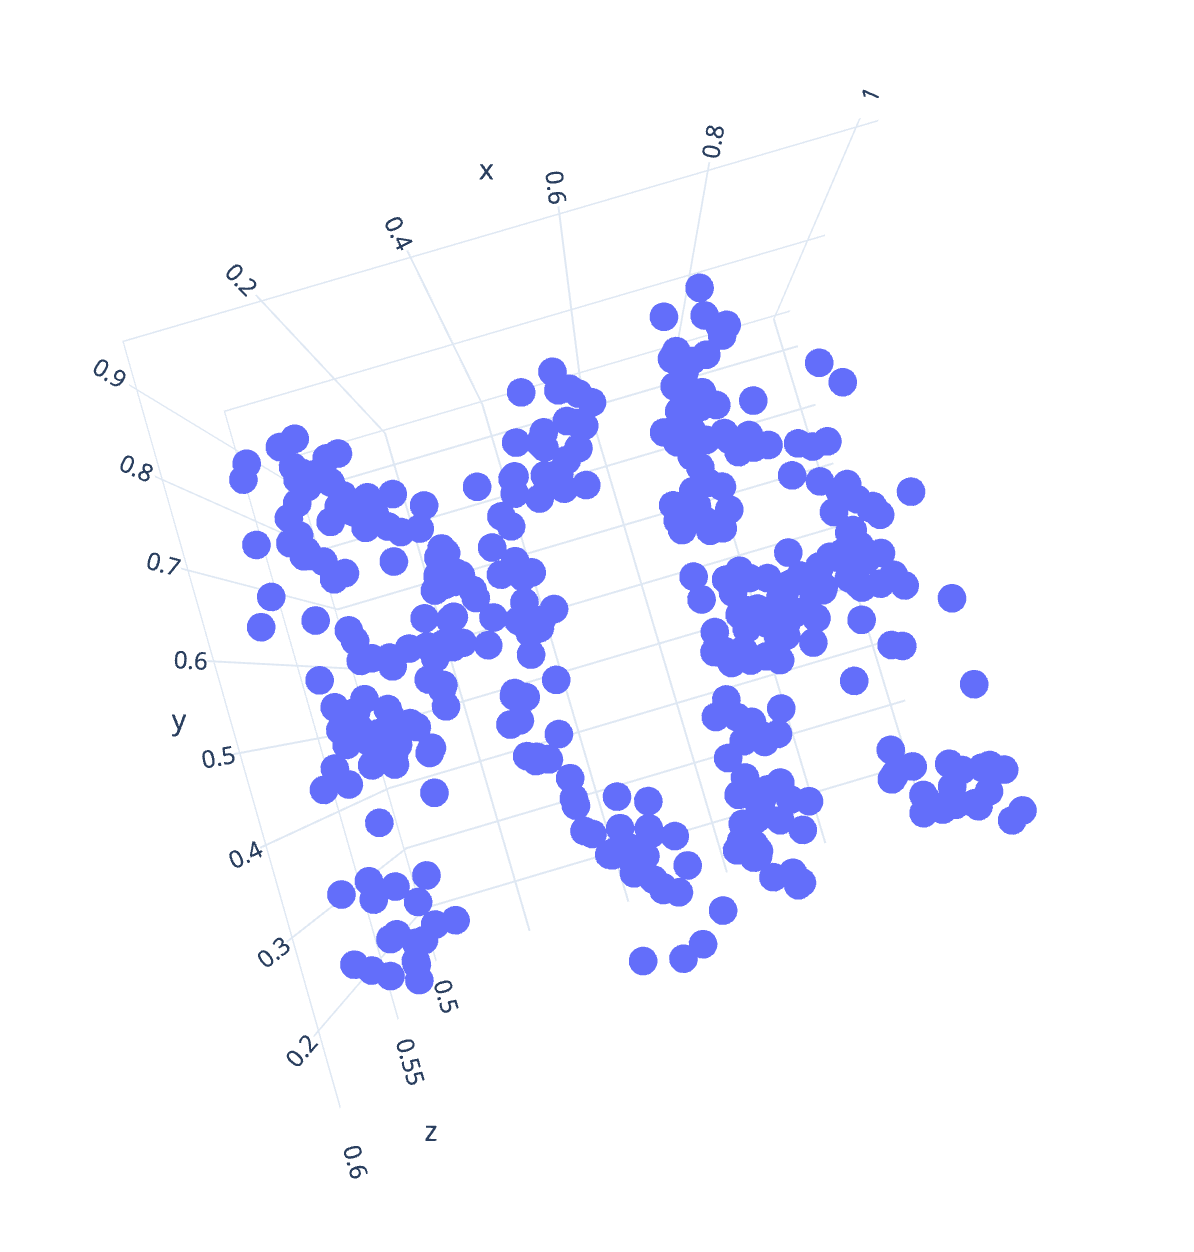
\includegraphics[scale=0.4]{pca-3d.png}
    \label{fig:pca3d}
\end{wrapfigure}

We want the data to be as spread out as possible. If we look from the direction parallel to the galactic plane, we see just a line. We lose one dimension, essentially keeping just a single coordinate for each star. (This is unfortunately exactly the perspective we see on the night sky: most stars are in the bright band we call the milky way, and we only see the outliers.) Among all possible projections, we attempt to find the one with the highest spread across the scatter plot. This projection may not be (and usually isn't) orthogonal to any axis; it may be projection to an arbitrary plane.

We again talk about two dimensional projection only for the sake of illustration. Imagine that we have ten thousand dimensional data and we would like, for some reason, keep just ten features. Yes, we can rank the features and keep the most informative, but what if these are correlated and tell us the same thing? Or what if our data does not have any target variable: with what should the "good features" be correlated? And what if the optimal projection is not aligned with the axes at all, so "good" features are combinations of the original ones?

We can do the same reasoning as above: we want to find a 10-dimensional (for the sake of examples) projection in which the data  points are as spread as possible.

How do we do this? Let's go back to our everyday's three dimensional world and think about how to find a two-dimensional projection.

Imagine you are observing a swarm of flies; your data are their exact coordinates in the room, so the position of each fly is described by three numbers. Then you discover that your flies actually fly in a formation: they are (almost) on the same line. You could then describe the position of each fly with a single number that represents the fly's position along the line. Plus, you need to know where in the space the line lies. We call this line the first principal component. By using it, we reduce the three-dimensional space into a single dimension.

After some careful observation, you notice the flies are a bit spread in one other direction, so they do not fly along a line but along a band. Therefore, we need two numbers, one along the first and one along the — you guessed it — second principal component.

It turns out the flies are actually also spread in the third direction. Thus you need three numbers after all.

Or do you? It all depends on how spread they are in the second and in the third direction. If the spread along the second is relatively small in comparison with the first, you are fine with a single dimension. If not, you need two, but perhaps still not three.

Let's step back a bit: why would one who carefully measured expressions of ten thousand genes want to throw most data away and reduce it to a dozen dimensions? The data, in general, may not and does not have as many dimensions as there are features. Say you have an experiment in which you spill different amounts of two chemicals over colonies of amoebas and then measure the expressions of 10.000 genes. Instead of flies in a three-dimensional space, you now profile colonies in a 10,000-dimensional space, the coordinates corresponding to gene expressions. Yet if expressions of genes depend only on the concentrations of these two chemicals, you can compute all 10,000 numbers from just two. Your data is then just two-dimensional.

\newpage

A technique that does this is called Principle Components Analysis, or PCA. The corresponding widget is simple: it receives the data and outputs the transformed data.

\begin{wrapfigure}{o}{0.6\textwidth}
    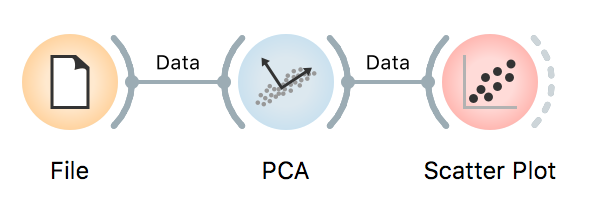
\includegraphics[width=\linewidth]{workflow-scatterplot.png}
    \label{fig:wf1}
\end{wrapfigure}

The widget allows you to select the number of components and helps you by showing how much information (technically: explained variance) you retain with respect to the number of components (brownish line) and the amount of information (explained variance) in each component.

\begin{figure}[h]
    \centering
    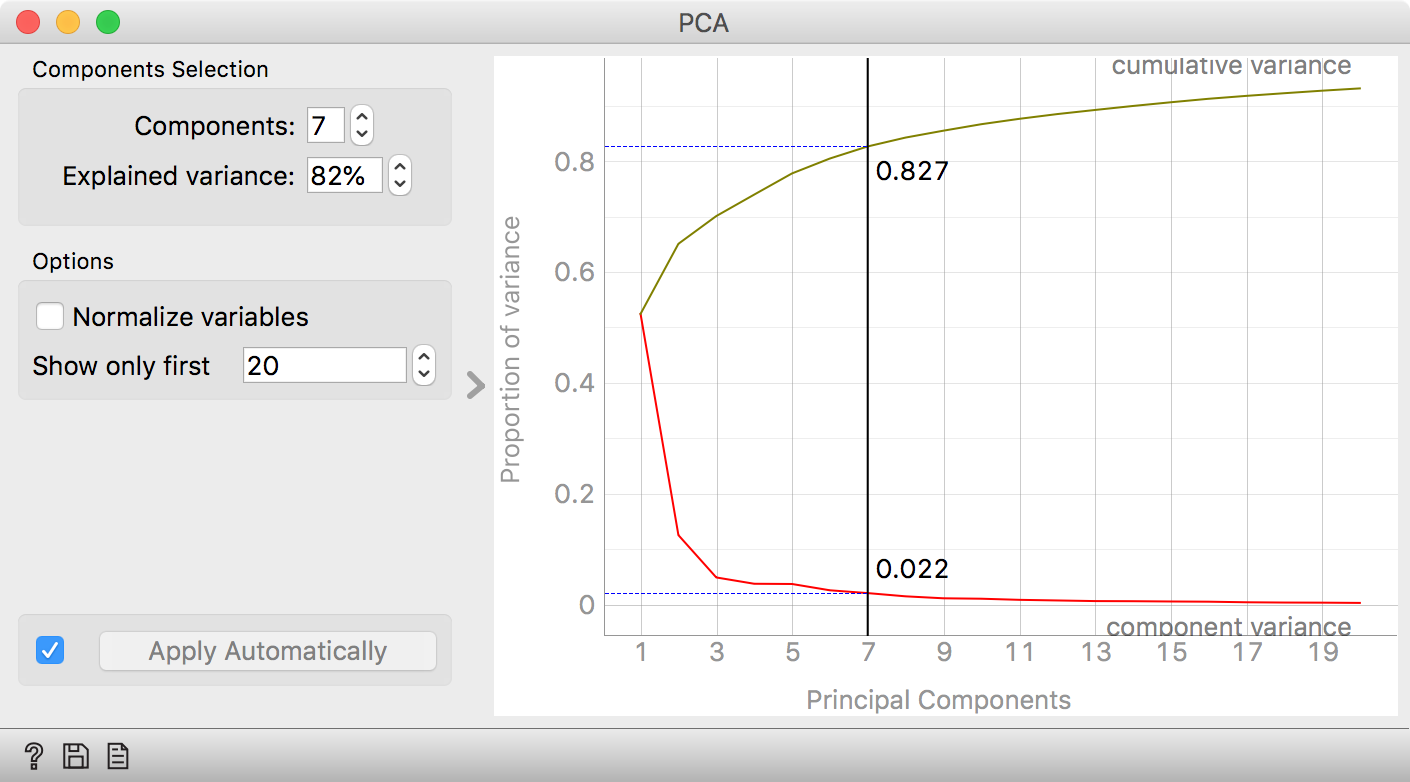
\includegraphics[width=\linewidth]{pca-scree.png}
    \caption{$\;$}
\end{figure}

The PCA on the left shows the scree diagram for brown-selected data. Set like this, the widget replaces the 80 features with just seven - and still keeping 82.7\% of information. (Note: disable "Normalize data" checkbox to get the same picture.) Let us see a scatter plot for the first two components.

\begin{figure}[h!]
    \centering
    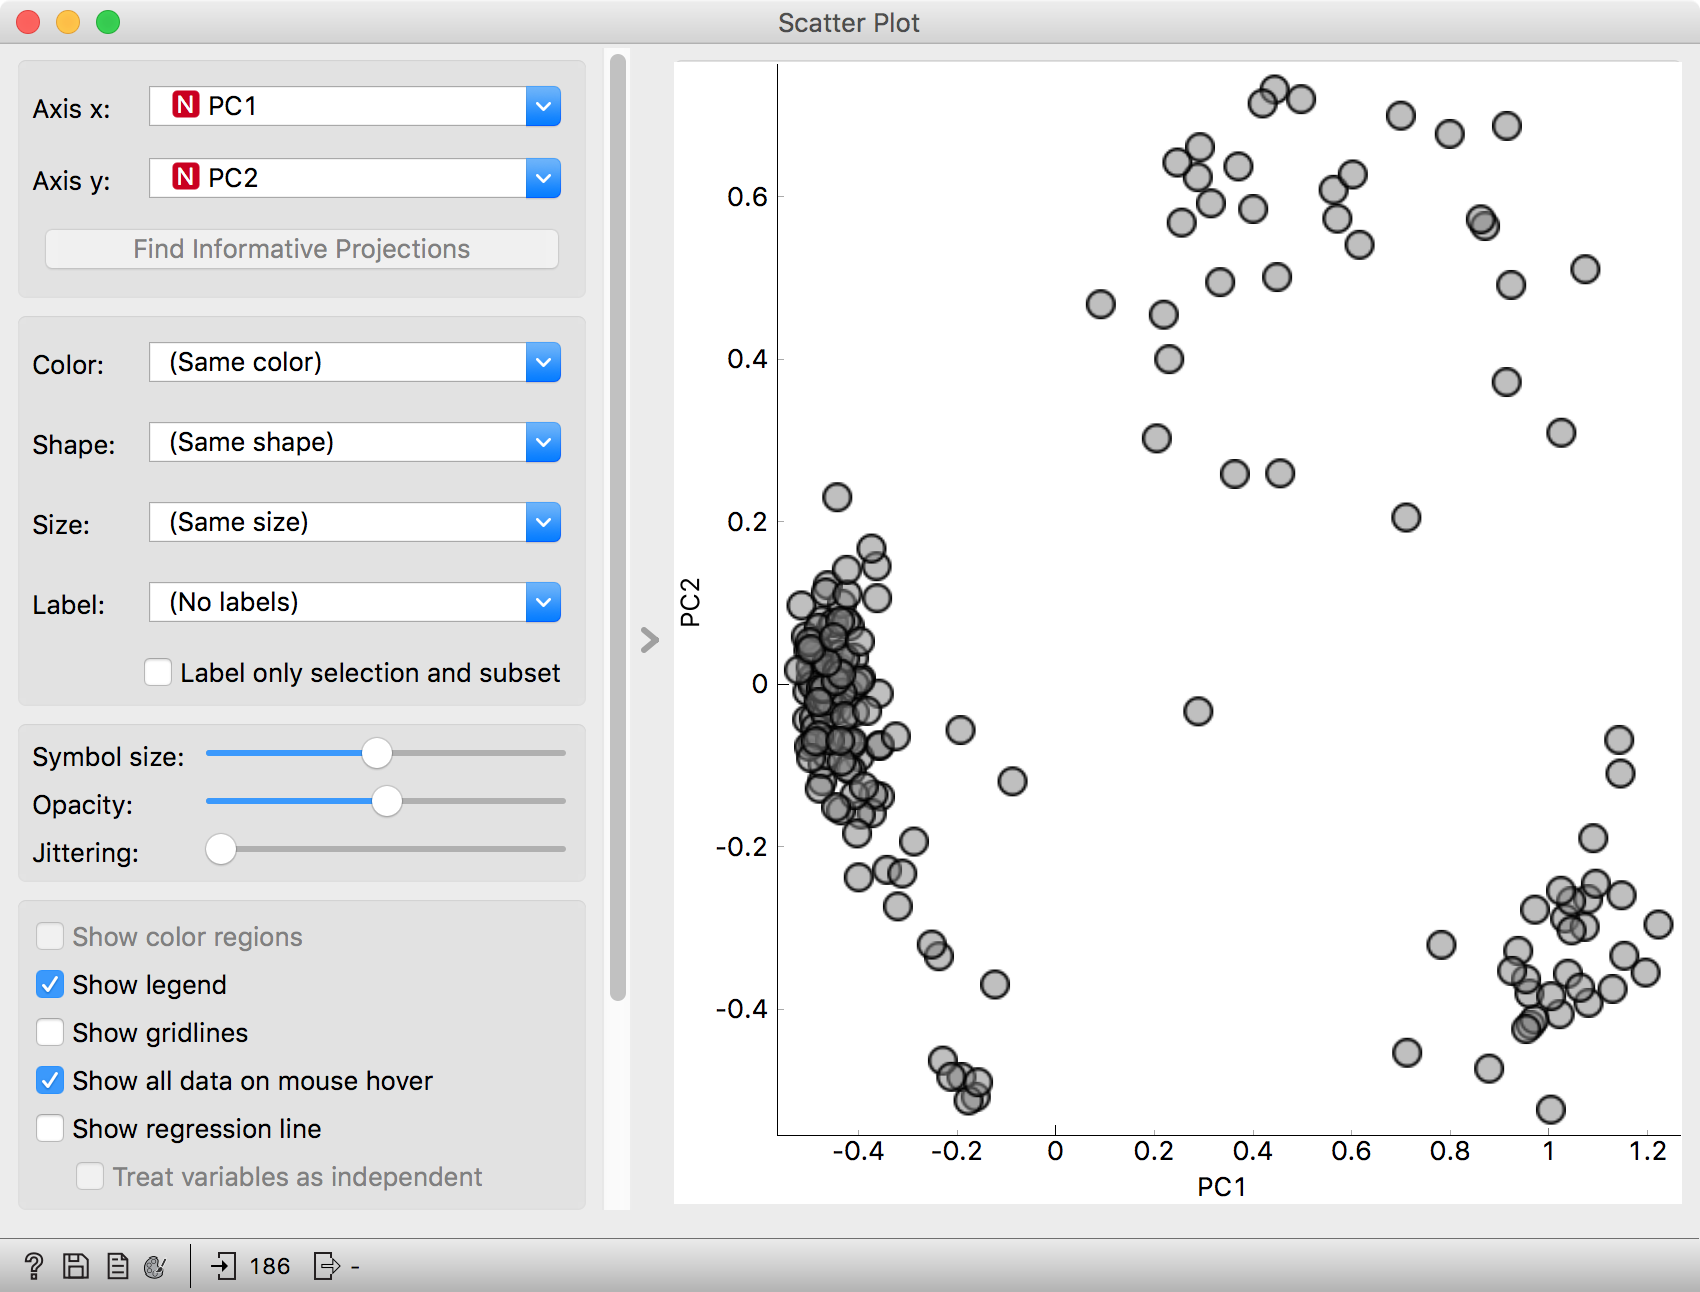
\includegraphics[width=\linewidth]{scatterplot-gray.png}
    \caption{$\;$}
\end{figure}

\newpage

The axes, PC1 and PC2, do not correspond to particular features in the original data, but to their linear combination. What we are looking at is a projection onto the plane, defined by the first two components. When you consider only two components, you can imagine that PCA put a hyperplane into multidimensional space and projecting all data into it.

Note that this is an unsupervised method: it does not care about the class. The classes in the projection may be be well separated or not. Let's add some colors to the points and see how lucky we are this time.

\begin{figure}[h]
    \centering
    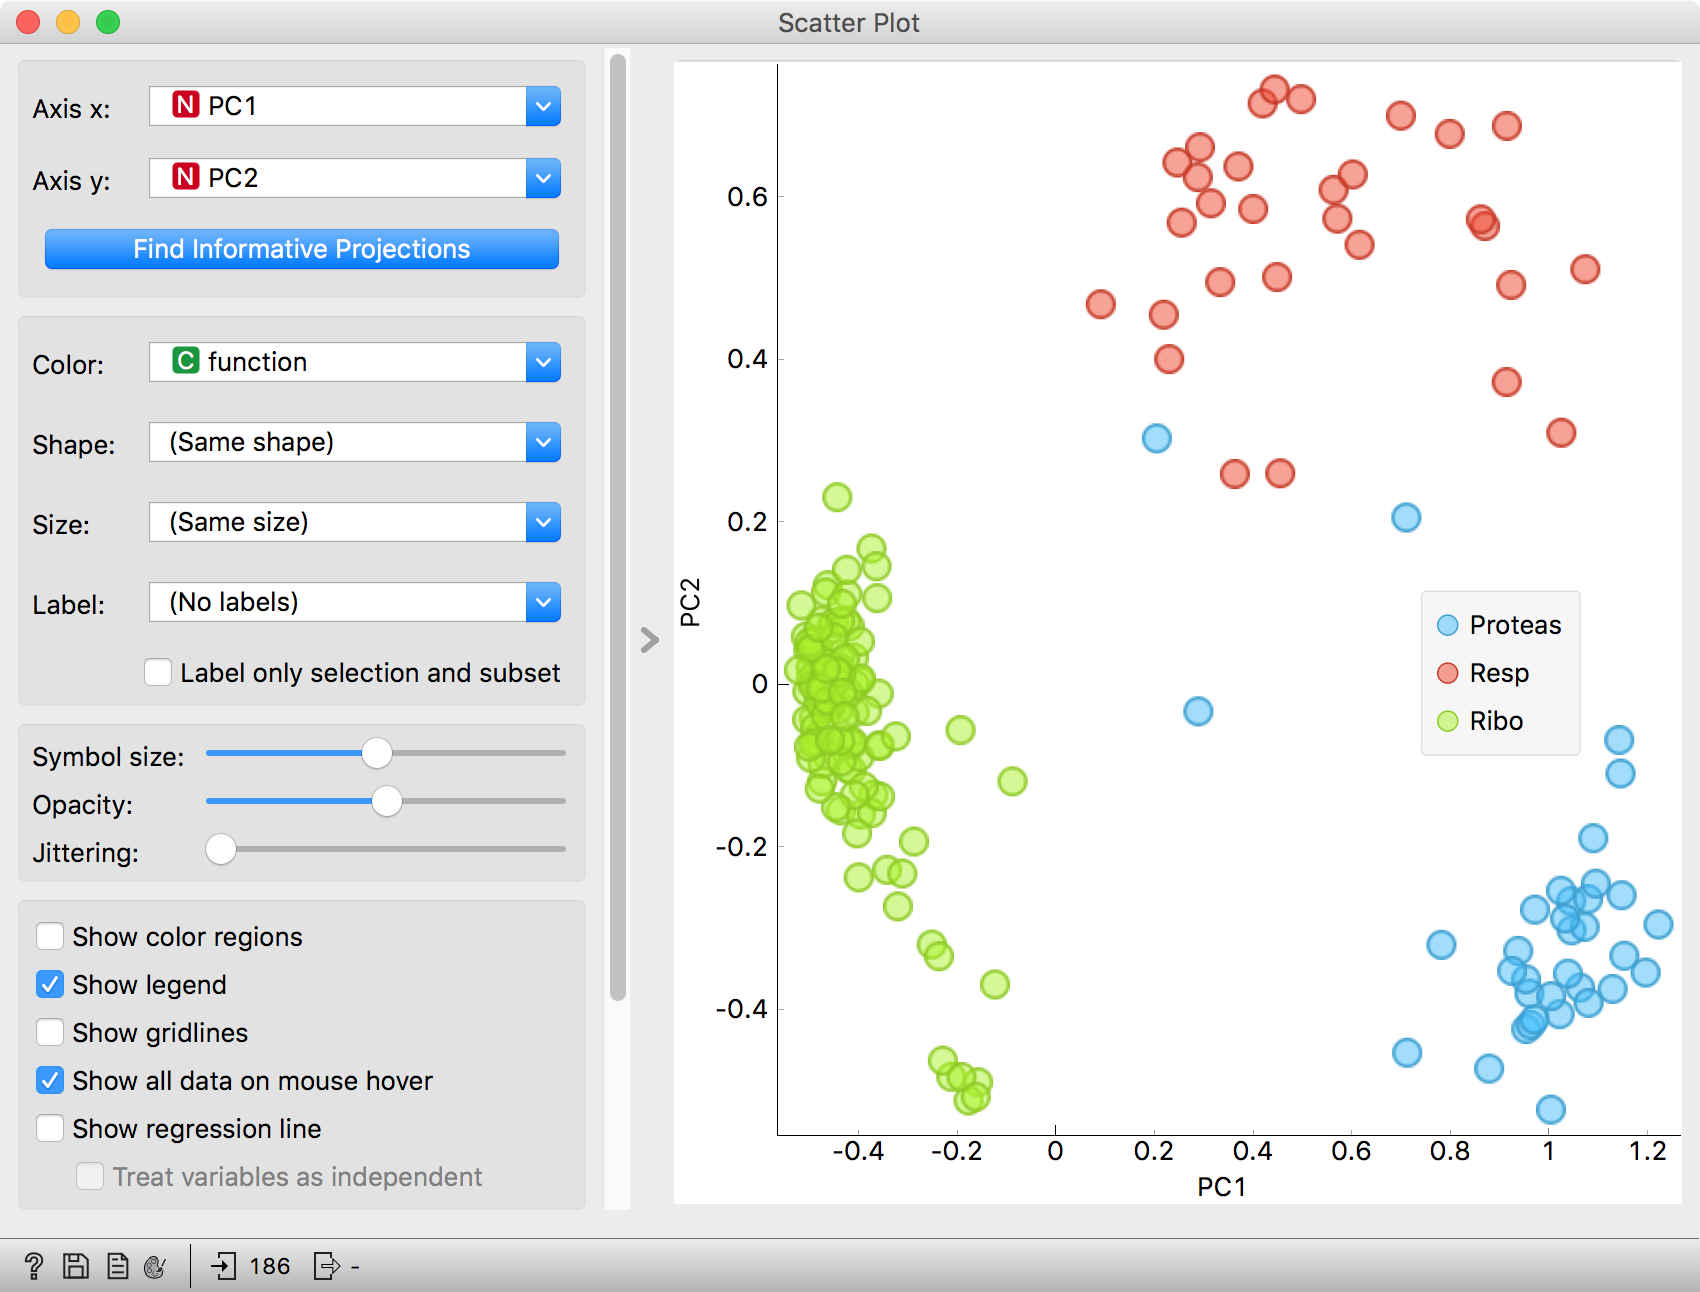
\includegraphics[width=\linewidth]{scatterplot-color.png}
    \caption{$\;$}
\end{figure}

The data separated so well that these two dimensions alone may suffice for building a good classifier. No, wait, it gets even better. The data classes are separated well even along the first component. So we should be able to build a classifier from a single feature!

\begin{figure*}[h]
    \centering
    \newcommand{\wf}{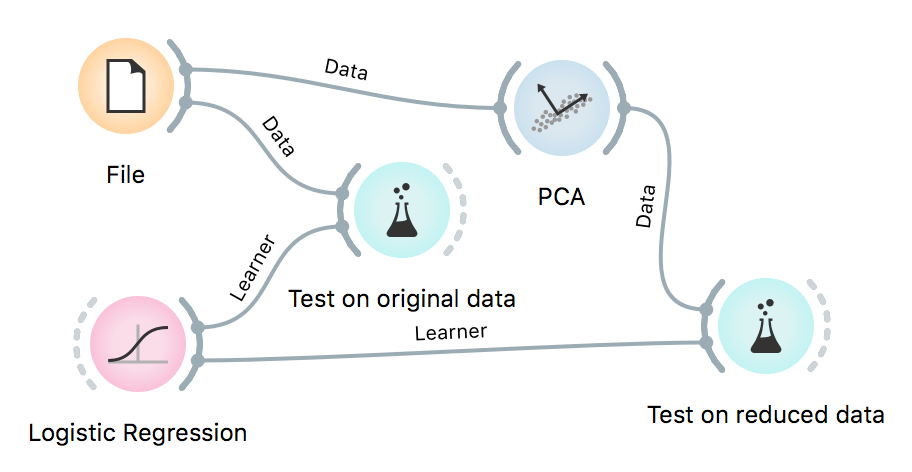
\includegraphics[scale=0.6]{workflow-testandscore.png}}
    \newcommand{\distrib}{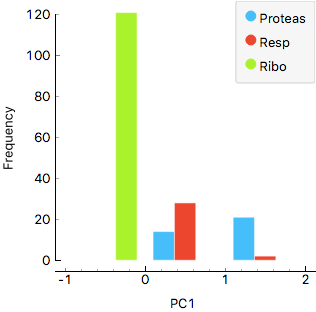
\includegraphics[scale=0.6]{distributions.png}}
    \infinitewidthbox{
    \stackinset{r}{-0.4\linewidth}{t}{+0.00\linewidth}{\distrib}{\wf}\hspace{8cm}
    }
\end{figure*}

\newpage

In the above schema we use the ordinary Test and Score widget, but renamed it to "Test on original data" for better understanding of the workflow.

On the original data, Logistic regression gets 98\% AUC and classification accuracy. If we select just single component in PCA, we already get a 93\%, and if we take two, we get the same result as on the original data.

PCA is thus useful for multiple purposes. It can simplify our data by combining the existing features to a much smaller number of features without losing much data. The directions of these features may tell us something about the data. Finally, it can find us good two-dimensional projections that we can observe in scatter plots.
